\documentclass[12pt]{article}

\usepackage[utf8]{inputenc}
\usepackage[T1]{fontenc}
\usepackage[polish,provide=*]{babel}
\usepackage{lmodern}
\usepackage{amsmath}
\usepackage{latexsym,amsfonts,amssymb,amsthm,amsmath}
\usepackage{enumitem}
\usepackage{hyperref}
\usepackage{float}
\usepackage{graphicx}
\usepackage{subcaption}
\usepackage{booktabs}
\graphicspath{{./images/}}

\setlength{\parindent}{0in}
\setlength{\oddsidemargin}{0in}
\setlength{\textwidth}{6.5in}
\setlength{\textheight}{8.8in}
\setlength{\topmargin}{0in}
\setlength{\headheight}{18pt}

\title{Pomiar krzywizny soczewki (pierścienie newtona)}
\author{Kacper Kłos}

\begin{document}

\maketitle

W tym raporcie przedstawimy metodę wyznaczania promienia krzywizny soczewki na podstawie badania pierścieni newtona. Wpierw ustawiliśmy soczewkę na szkle pod mikroskopem, dopasowaliśmy skalę na podstawie papieru milimetrowego. Następnie naświetlaliśmy soczewkę światłem koloru czerwonego, zielonego i niebieskeigo. Później mierzyliśmy średnice \(k\)-tego pierścienia newtona oraz dopasowaliśmy linię do relacji \(D_k^2(k)\). Następnie przebadaliśmy widmo generowane przez używaną lampę w celu wyznaczenia długości fali jaka pada na soczewkę. Przy pomocy otrzymanych danych wyznaczyliśmy promień krzywizny dla każdego z kolorów, a następnie przy użyciu średniej ważonej wyznaczyliśmy finalny promień \(R = (6{,}613 \pm 0{,}014) \, \mathrm{m}\).

\newpage


\section{Wyniki Pomierów}
W tabli~\ref{tab:rgb_measurements_reversed} widoczne są wyniki jakie uzyskaliśmy mierząc średnice \(k\)-tego pierścienia newtona mierząc do jego środka geometrycznego.
\begin{table}[H]
	\centering
	\begin{tabular}{c|cc|cc|cc}
		\toprule
        Nr & \multicolumn{2}{c|}{\(D_r \, [\mathrm{cm}]\)} & \multicolumn{2}{c|}{\(D_g \, [\mathrm{cm}]\)} & \multicolumn{2}{c}{\(D_b \, [\mathrm{cm}]\)}                            \\
		   & 1                            & 2                            & 1                           & 2      & 1      & 2      \\
		\midrule
		1  & 0{,}33                       & 0{,}32                       & 0{,}29                      & 0{,}30 & 0{,}22 & 0{,}22 \\
		2  & 0{,}44                       & 0{,}44                       & 0{,}39                      & 0{,}40 & 0{,}34 & 0{,}34 \\
		3  & 0{,}52                       & 0{,}52                       & 0{,}47                      & 0{,}48 & 0{,}42 & 0{,}42 \\
		4  & 0{,}60                       & 0{,}60                       & 0{,}54                      & 0{,}54 & 0{,}49 & 0{,}49 \\
		5  & 0{,}67                       & 0{,}67                       & 0{,}59                      & 0{,}60 & 0{,}55 & 0{,}55 \\
		6  & 0{,}74                       & 0{,}73                       & 0{,}65                      & 0{,}66 & 0{,}61 & 0{,}61 \\
		7  & 0{,}78                       & 0{,}78                       & 0{,}70                      & 0{,}70 & 0{,}66 & 0{,}66 \\
		8  & 0{,}84                       & 0{,}84                       & 0{,}75                      & 0{,}76 & 0{,}71 & 0{,}71 \\
		9  & 0{,}88                       & 0{,}88                       & 0{,}79                      & 0{,}79 & 0{,}75 & 0{,}75 \\
		10 & 0{,}92                       & 0{,}92                       & 0{,}84                      & 0{,}84 & 0{,}79 & 0{,}79 \\
		\bottomrule
	\end{tabular}
	\caption{Pomiery średnicy \(n\)-tego pierścieni newtona dla świateł o kolorach \(D_r\)-czerwony, \(D_g\)-zielony, \(D_b\)-niebieski przy dwóch seriach pomiarowych. Numery nieprzyste odpowiadają jasnym pierścienią, a parzyste ciemnym}
	\label{tab:rgb_measurements_reversed}
\end{table}

Za błąd pomiarowy uznajemy \(0{,}01 \, \mathrm{cm}\) w przypadku wszystkich pierścieni poza pierwszymi 2 pierścieniami jasnymi.
Dla dwóch pierszyszych jasnych pierścienie we wszystkich pomiarach zakładamy błąd w okolicach \(0{,}02 \, \mathrm{cm}\) jako że były one znacznie grubsze a nasze pomiary mierzyły śrdnice wyznaczaną przez środek geometryczny, który w przypadku funkcji kwadratowej nie koniecznie się pokrywa.

Nasępnie do tych dancyh możemy dopasować prostą wyznaczoną w instrukcji~\cite{skrypt} do zmierzonych średnic z tabli~\ref{tab:rgb_measurements_reversed} aby wyznaczyć współczynnik kierunkowy.
\begin{equation}
	D_k^2 = \frac{k \lambda R}{8}
	\label{eq:radious}
\end{equation}
Gdzie \(r_k\) jest promieniem \(k\)-tego pierścienia newtona, \(R\) promień krzywizny soczewki, \(\lambda\) długość fali.

\begin{figure}[H]
	\centering
	\begin{subfigure}{0.3\textwidth}
		\centering
		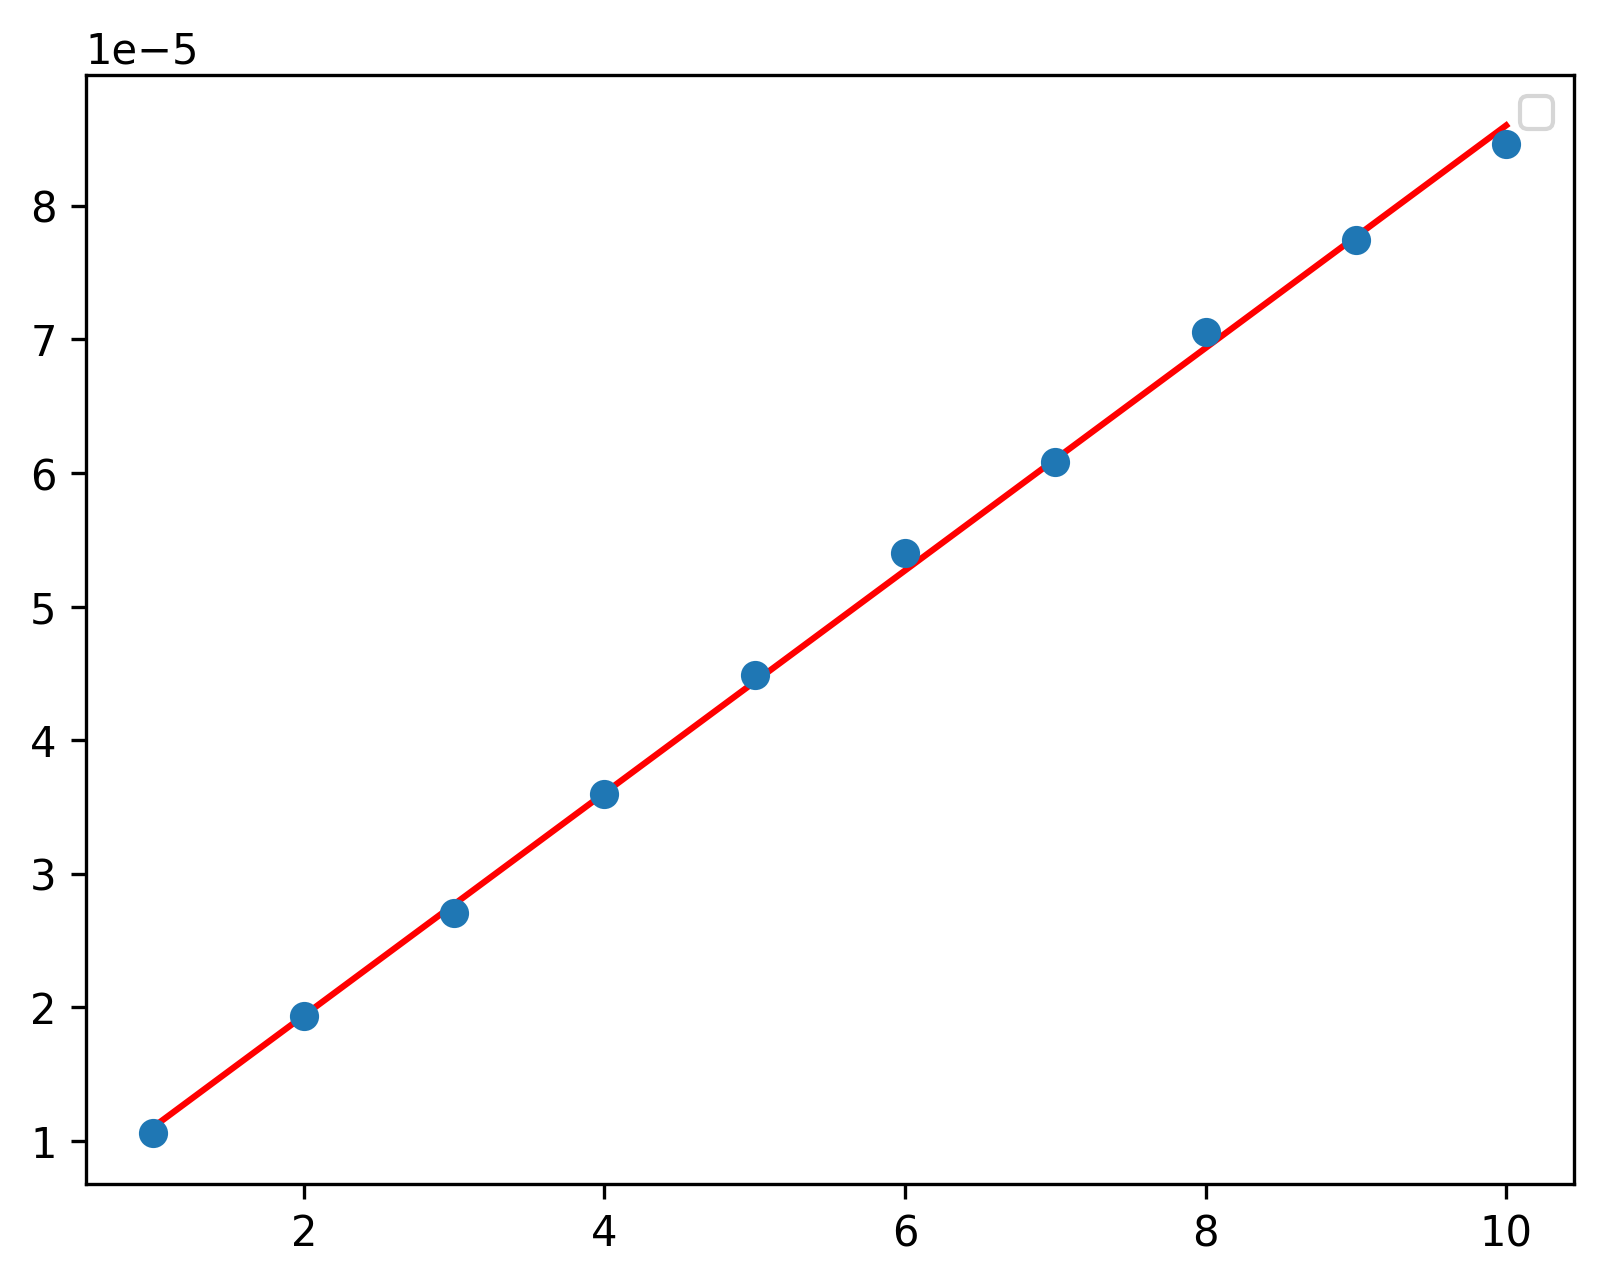
\includegraphics[width=\linewidth]{red}
		\caption{czerwony}
		\label{fig:red_line}
	\end{subfigure}
	\hfill
	\begin{subfigure}{0.3\textwidth}
		\centering
		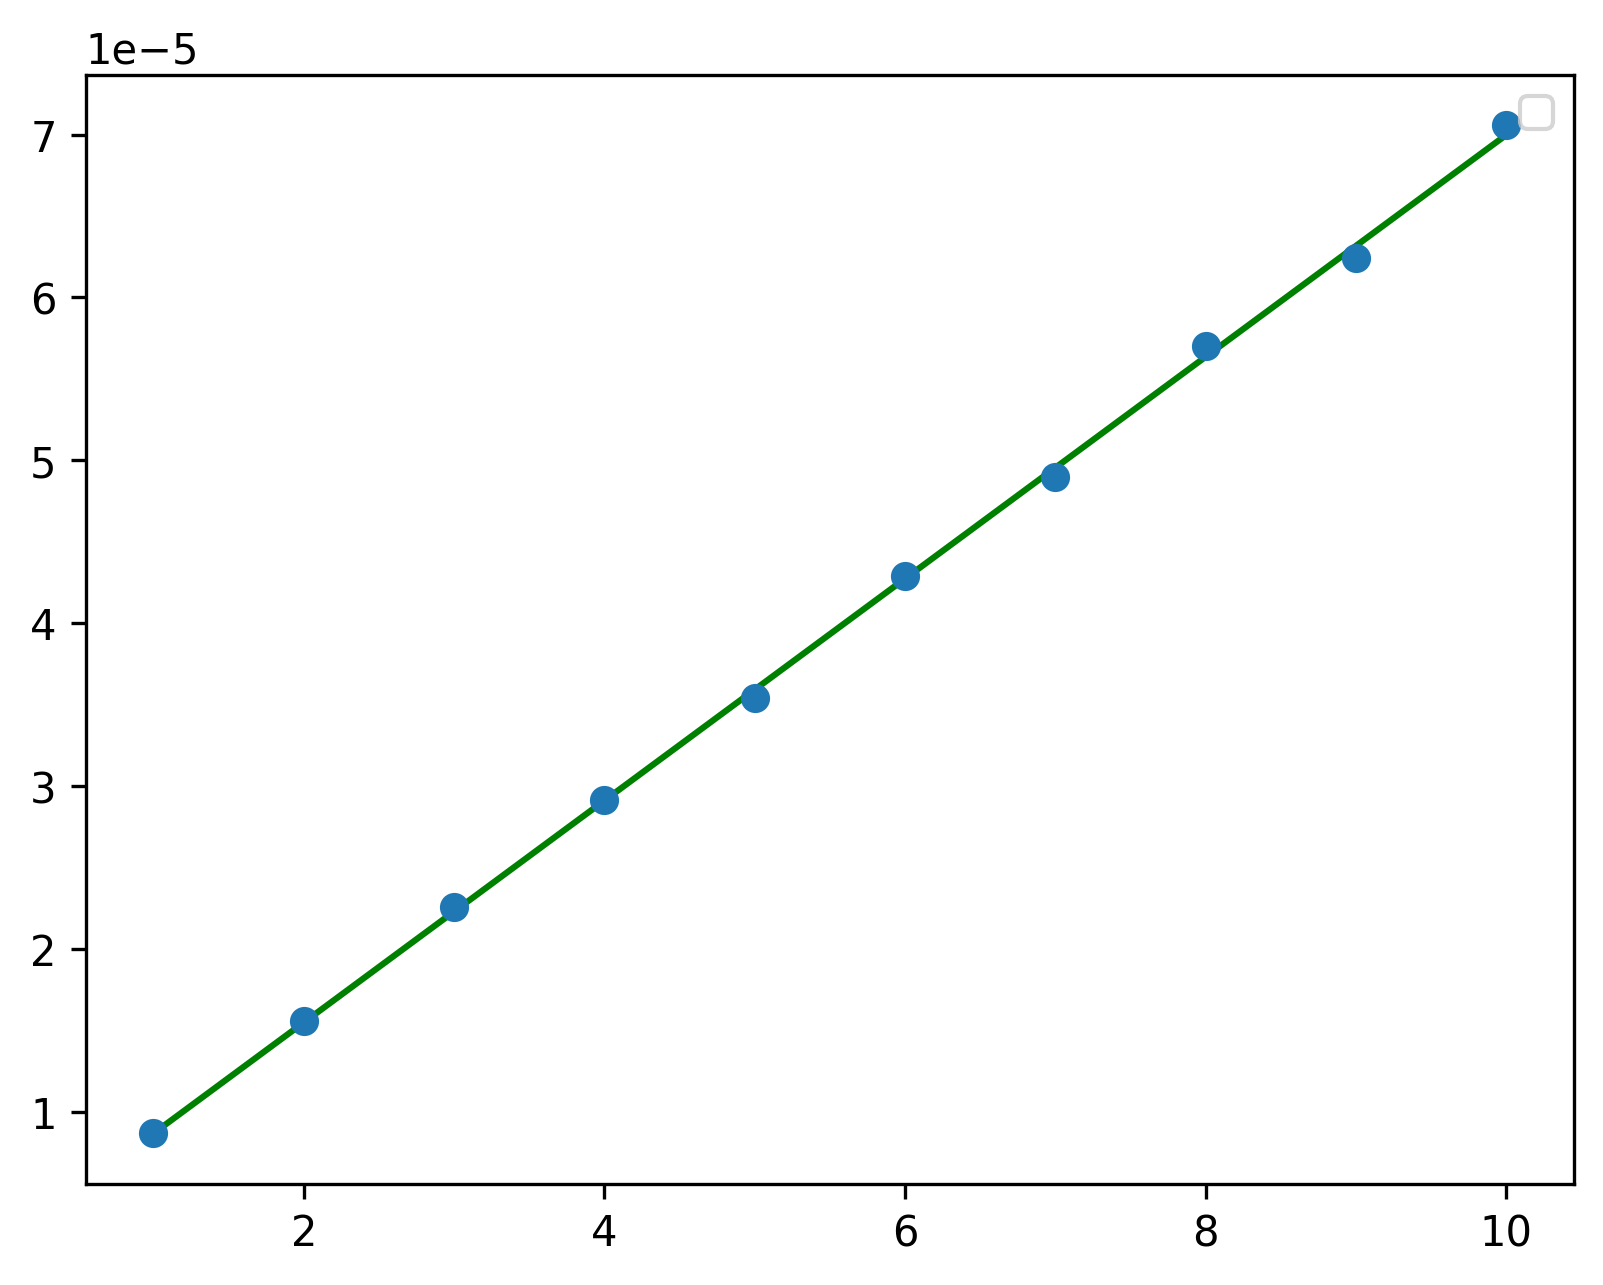
\includegraphics[width=\linewidth]{green}
		\caption{zielony}
		\label{fig:green_line}
	\end{subfigure}
	\hfill
	\begin{subfigure}{0.3\textwidth}
		\centering
		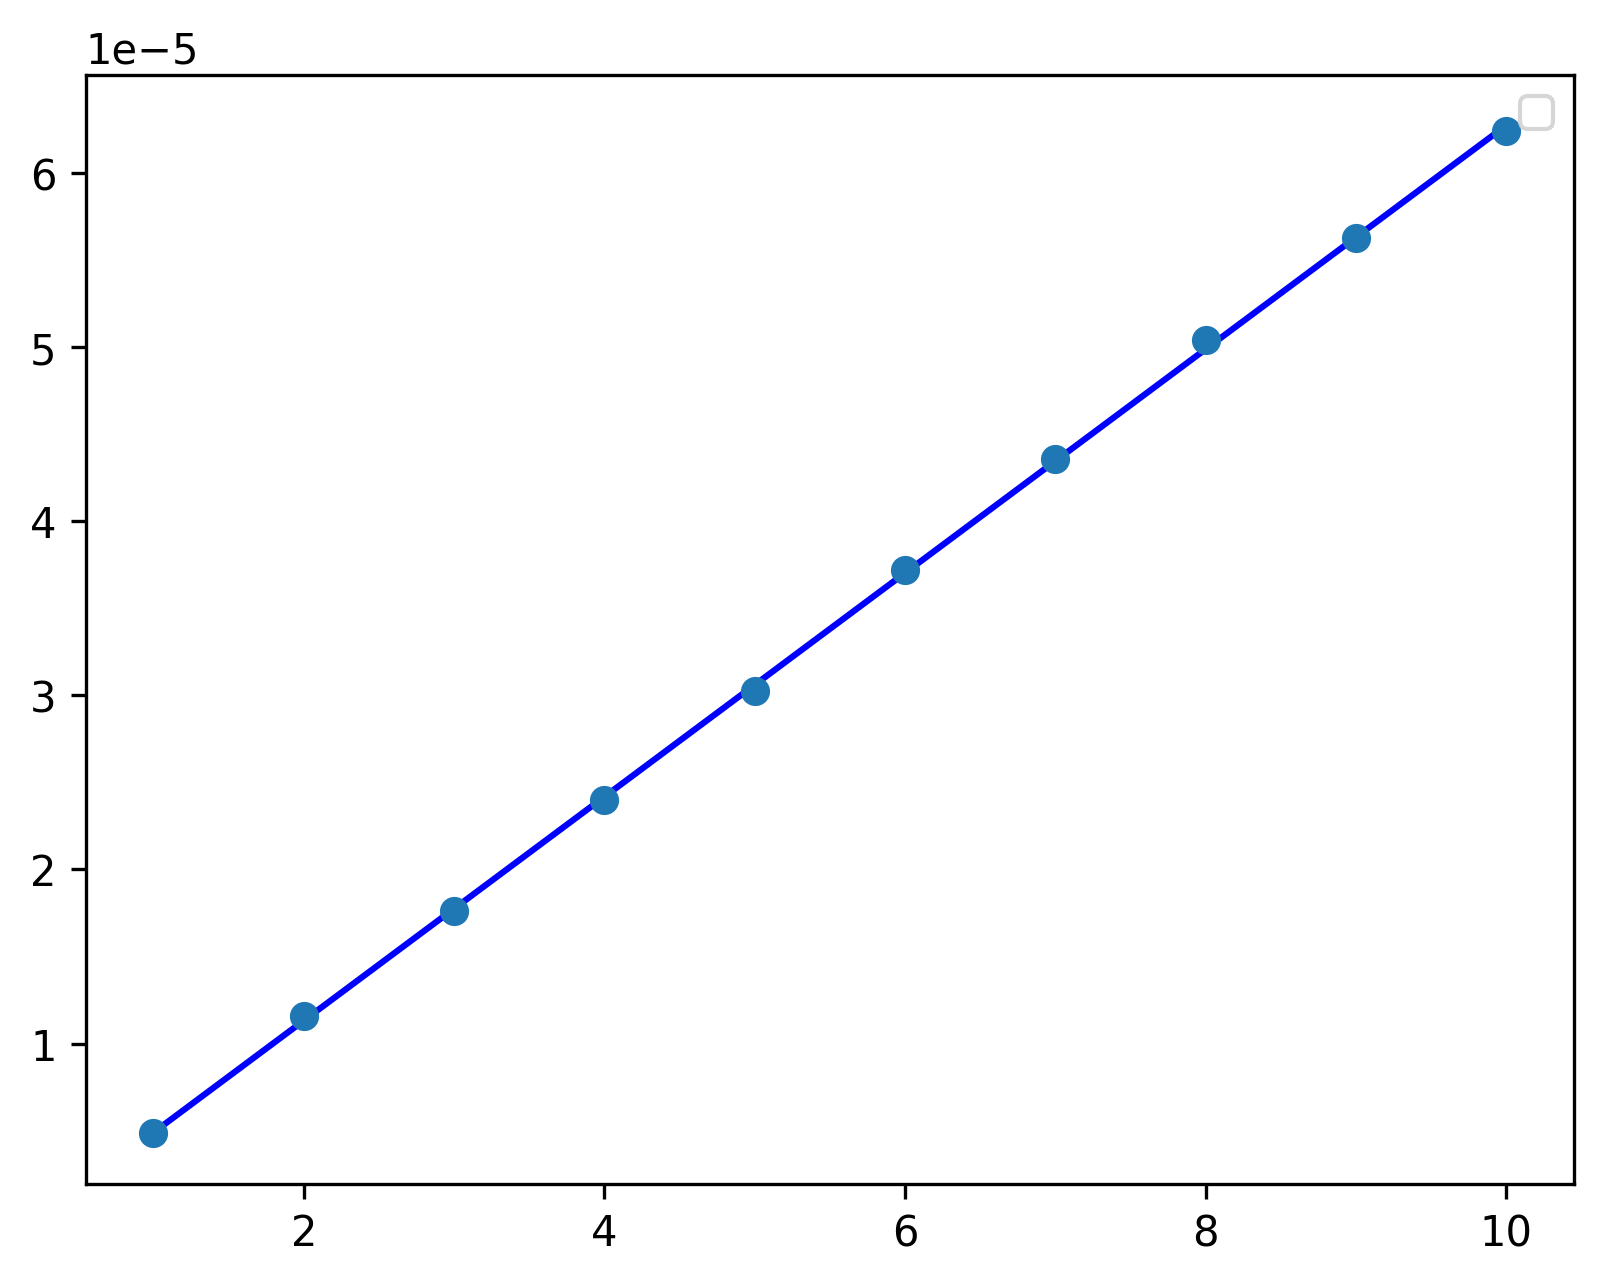
\includegraphics[width=\linewidth]{blue}
		\caption{niebieski}
		\label{fig:blue_line}
	\end{subfigure}
	\caption{Punkty pomiarowe oraz dopasowanie liniowe do średnicy pierścieni newtona dla różnych kolorów}
	\label{fig:line_graphs}
\end{figure}
Dopasowanie do równania \(D_k^2 = a k + b\) daje wyniki:
\begin{table}[H]
	\centering
	\begin{tabular}{c|cc}
		\toprule
		kolor     & $a$                             & $b$                            \\
		\midrule
		czerwony  & \((210 \pm 18) \times 10^{-9}\) & \((59 \pm 7) \times 10^{-9}\)  \\
		zielony   & \((170 \pm 10) \times 10^{-9}\) & \((49 \pm 4) \times 10^{-9}\)  \\
		niebieski & \((161 \pm 8) \times 10^{-9}\)  & \((-37 \pm 3) \times 10^{-9}\) \\
		\bottomrule
	\end{tabular}
	\caption{Współczynniki kierunkowe dopasowane do zależności \(r_k^2(k)\) dla różnych kolorów światła.}
	\label{tab:lines_params}
\end{table}

Aby wekstrachować z otrzymanych współczynników promień krzywizny soczewki potrzebujemy dokładnie wyznaczyć długość fali światła dla badanego koloru. Aby to zrobić musimy przeanalizować wykresy zależności intensywności od długości fali dla światła które używaliśmy. W tym celu dla każdego z wykresów zależności intensywności od długości fali wyznaczymy długość fali na podstawie punktu dla którego jest maksymalna intensywność. Następnie wyznaczymy dla jakiej długości fal przyjmowane są wartości na poziomie \(50\%\) maksymalnej intensywności, a błąd uznamy za większą z różnic między punktem z \(50\%\) a maksymalną intensywnością.
\begin{figure}[H]
	\centering
	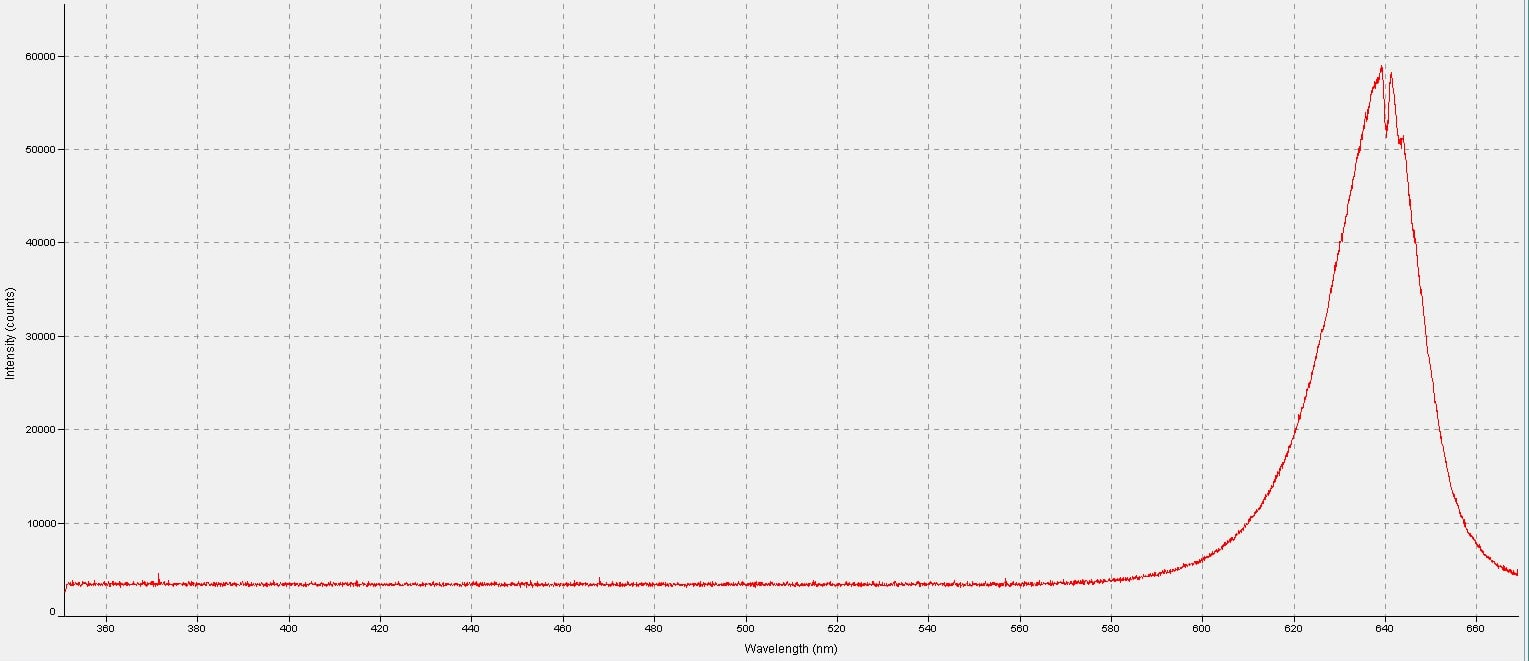
\includegraphics[scale=0.3]{red_wavelength}
	\caption{Wykres intensywności światła od długości fali}
	\label{fig:red_wavelength}
\end{figure}
Na wykresie~\ref{fig:red_wavelength} dla światła czerwonego widzimy lekkie zakłócenia, lecz niewątpliwie maksimum intensywności \(I \approx 60000\) napotykamy przy fali długości \(\lambda_{\mathrm{red}} = 640 \, \mathrm{nm}\), podczas gdy połowę tej intensywności napotykamy dla punktów \(\lambda_{\mathrm{r1}} = 628 \, \mathrm{nm}\) oraz \(\lambda_{\mathrm{r2}} = 650 \, \mathrm{nm}\). Dlatego dla światła czerwonego otrzymujemy wynik \(\lambda_{\mathrm{red}} = 640 \pm 12 \, \mathrm{nm}\).

\begin{figure}[H]
	\centering
	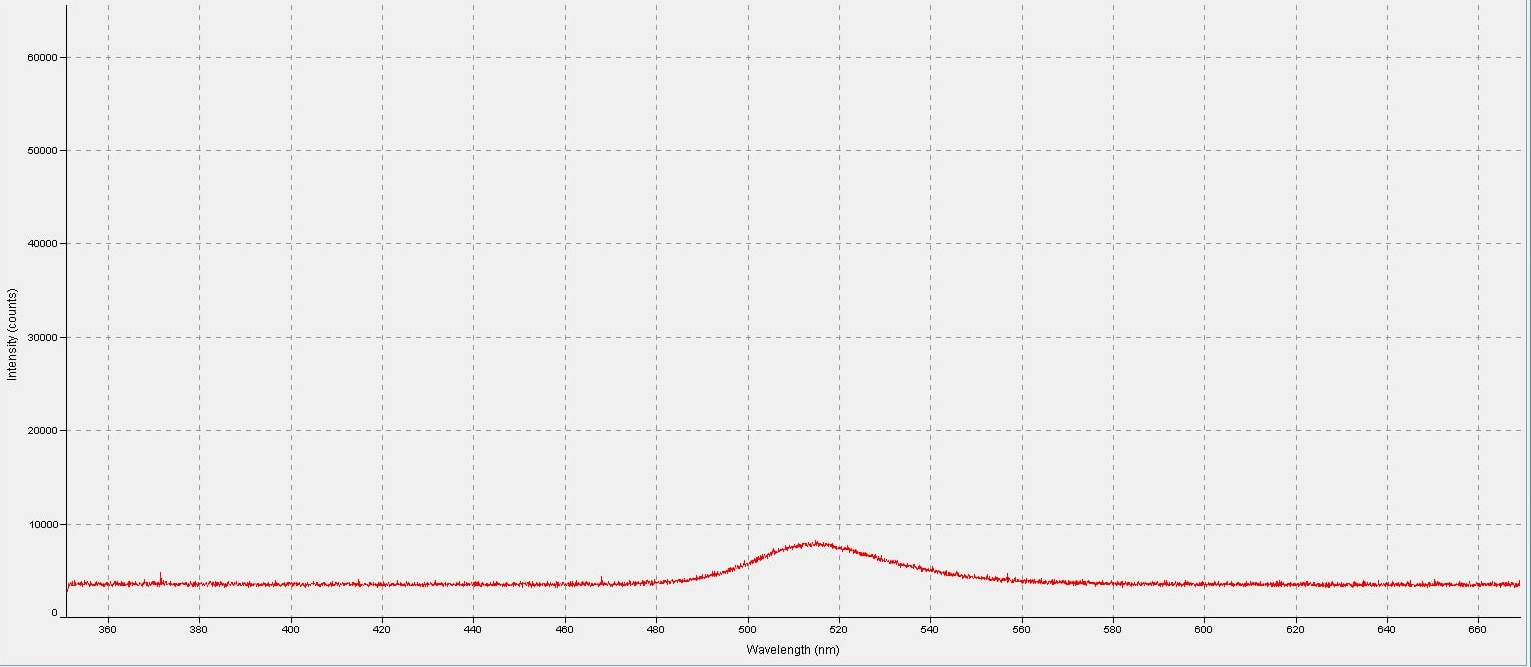
\includegraphics[scale=0.3]{green_wavelength}
	\caption{Wykres intensywności światła od długości fali}
	\label{fig:green_wavelength}
\end{figure}
Analogiczną analize wykonujemy dla światła zielonego widocznego na wykresie~\ref{fig:green_wavelength}. Szczyt przyjmowany dla intensywności \(I \approx 8000\) i długości fali \(\lambda_{\mathrm{green}} = 515 \, \mathrm{nm}\) jest znacznie mniej wyrazisty niż w przypadku światła czerwonego. Połowę maksymalnej intensywności napotykamy dla punktów \(\lambda_{\mathrm{g1}} = 495 \, \mathrm{nm}\) oraz \(\lambda_{\mathrm{g2}} = 540 \, \mathrm{nm}\). Także dla światła zielonego otrzymujemy wynik \(\lambda_{\mathrm{green}} = 515 \pm 25 \, \mathrm{nm}\) z dwa razy większym błędem dla światła czerwonego.

\begin{figure}[H]
	\centering
	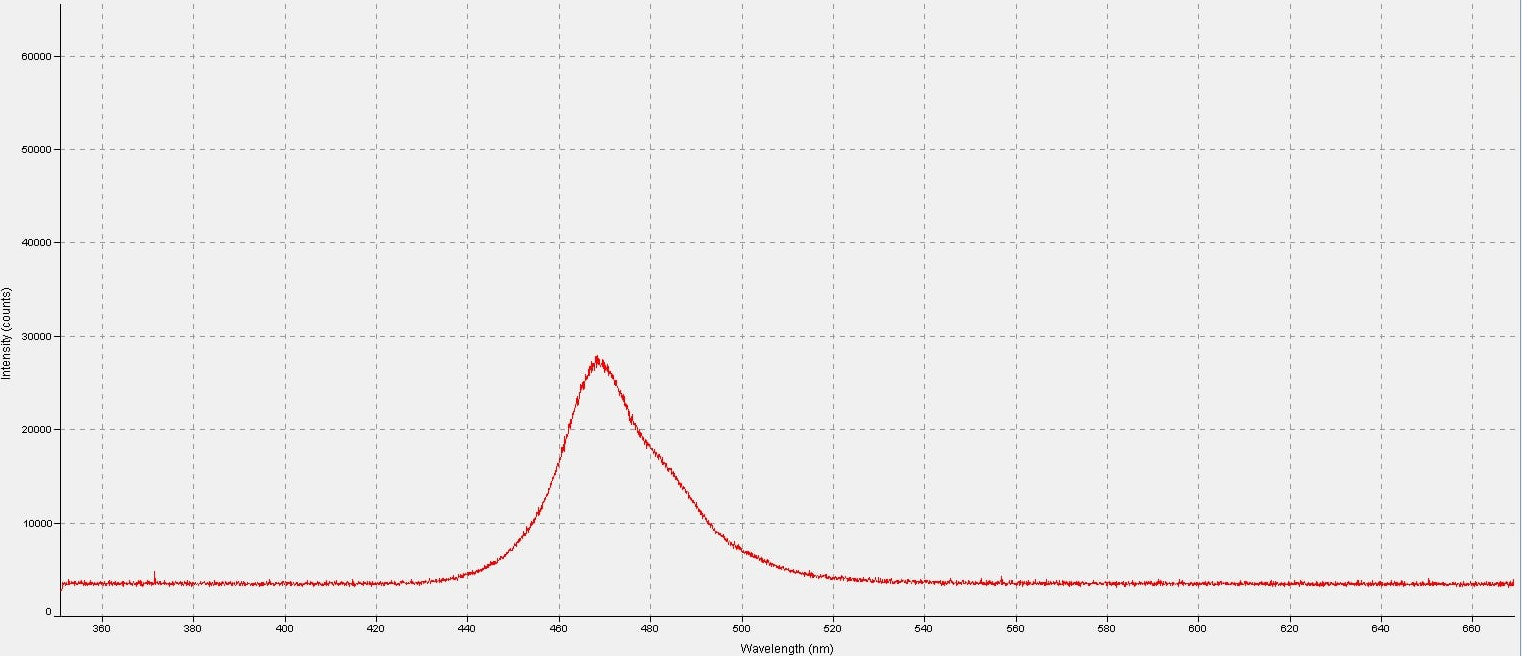
\includegraphics[scale=0.3]{blue_wavelength}
	\caption{Wykres intensywności światła od długości fali}
	\label{fig:blue_wavelength}
\end{figure}
Finalnie analizując wykres~\ref{fig:blue_wavelength} dla światła niebieskiego. Szczyt napotykamy dla intensywności \(I \approx 28000\) i długości fali \(\lambda_{\mathrm{blue}} = 468 \, \mathrm{nm}\). Połowę maksymalnej intensywności napotykamy dla punktów \(\lambda_{\mathrm{b1}} = 455 \, \mathrm{nm}\) oraz \(\lambda_{\mathrm{g2}} = 488 \, \mathrm{nm}\). Podsumowując wyniki dla światła niebieskiego \(\lambda_{\mathrm{blue}} = 468 \pm 20 \, \mathrm{nm}\) będąc bardziej dokładnym od światła zielonego lecz mniej od światła czerwonego.

Finalnie otrzymujemy
\begin{table}[H]
	\centering
	\begin{tabular}{c|c}
		\toprule
		kolor     & \(\lambda \, [\mathrm{nm}]\) \\
		\midrule
		czerwony  & \(640 \pm 12\)               \\
		zielony   & \(515 \pm 25\)               \\
		niebieski & \(468 \pm 20\)               \\
		\bottomrule
	\end{tabular}
	\caption{Wyznaczone długości fal dla badanych kolorów}
	\label{tab:wavelength}
\end{table}

Korzystając z danych z tabel~\ref{tab:lines_params}~\ref{tab:wavelength} oraz wzoru \eqref{eq:radious} możemy wyznaczyć promień krzywizny soczewki za pomocą wzoru
\[
	R = 8\frac{a}{\lambda}
\]
Oraz błąd
\[
	u(R) = 8\frac{a}{\lambda} \sqrt{(\frac{u(\lambda)}{\lambda})^2 + (\frac{u(a)}{a})^2}
\]
Przy pomocy tych wzorów otrzymujemy

\begin{table}[H]
	\centering
	\begin{tabular}{c|c}
		\toprule
		kolor     & \(R [\mathrm{m}]\)    \\
		\midrule
		czerwony  & \(6{,}58 \pm 0{,}14\) \\
		zielony   & \(6{,}59 \pm 0{,}4\)  \\
		niebieski & \(6{,}86 \pm 0{,}3 \) \\
		\bottomrule
	\end{tabular}
	\caption{Wyznaczone promienie soczewki dla danych kolorów}
	\label{tab:radious}
\end{table}

Biorąc średnią ważoną z tabeli~\ref{tab:radious}
\[
	R = \frac{\sum_i \frac{R_i}{u(R)_i^2}}{\sum_i \frac{1}{u(R)_i^2}}, \quad u(R) = \frac{1}{\sum_i \frac{1}{u(R)_i^2}}
\]
Finalnie korzystając z tych wzorów otrzymujemy promień
\[
	R = 6{,}613 \pm 0{,}014
\]
Możemy zauważyć że główną przyczyną błędów w naszych pomiarach jest błąd pochodzący z długości fali. Światło czerwone posiadało największy błąd dopasowaniaa, lecz z powodu najmniejszego błędu długości fali jest to najdokładniejszy pomiar promienia. Widzimy że najbardziej odbiegający wynik jest dla światła niebieskiego, podczas tych pomiarów musiał się wkraść niespodziewany błąd który widzimy szczególnie z powodu że parametr \(b\) jest ujemny. Obecny jest też błąd systematyczny spowodowany kalibracją skali do papieru mimiletrowego.

\newpage


\begin{thebibliography}{1}

	\bibitem{skrypt}
	\emph{Interferencyjny Pomiar Krzywizny Soczewki (Pierścienie Newtona)}, Uniwersytet Warszawski.

\end{thebibliography}


\end{document}
